%!TEX root = ../main.tex

\chapter{Literature Review}\label{cha:literature}

As described in Chapter \ref{cha:introduction}, the Prisoner's Dilemma is a very popular model in game theory and there have been many papers written about the subject.
The game has been applied to many different research areas is often used to model systems in biology \cite{Sigmund1999}, sociology \cite{Franken2005}, psychology \cite{Ishibuchi2005}, and economics \cite{Chong2005}.
The start of this chapter will give a brief overview of the literature and particularly relevant work will be highlighted.
This is followed by an outline of how Axelrod's work is currently being reproduced by an open-source community.
Finally, an introduction to fingerprinting (a technique used for identify
similar strategies) and some necessary definitions and theorems are given at the end of the chapter.


\section{Background}\label{sec:axelrodoriginal}

The political scientist Robert Axelrod held the first IPD tournament in 1980 \cite{Axelrod1980a}.
Many well-known game theorists were invited to submit strategies that would compete against each other in a round robin style format.
All strategies also competed against a random strategy (that would randomly choose between $C$ and $D$) and a copy of themselves.
All strategies knew that the length of each game was 200 moves, and the whole tournament was repeated 5 times for reliability.
Out of the 13 strategies that were entered, TitForTat was announced as the winner and was submitted by Professor Anatol Rapoport from the Department of Psychology of the University of Toronto \cite{Rapoport2015}.

TitForTat is a very simple strategy (see Section \ref{ssec:stra_titfortat}) and as explained in \cite{Axelrod1980b}, it won because of three defining characteristics:

\begin{itemize}
    \item `Niceness' - A strategy is said to be nice if it is not the first to defect.
    \item `Provocability' - Immediately after an opponent defects, the strategy should defect in retaliation.
    \item `Forgiveness' - The strategy is willing to continue with mutual cooperation even after some defections.
\end{itemize}

Axelrod's second tournament \cite{Axelrod1980b} saw a dramatic increase in terms of size, with 62 strategies being entered from 6 different countries (the strategy Random was also included).
The contestants ranged from a 10-year-old computer hobbyist to professors of computer science, economics, psychology, mathematics, sociology, political science and evolutionary biology.
The countries represented were the United States, Canada, Great Britain, Norway, Switzerland, and New Zealand.
Despite the fact that all contestants had full knowledge of the previous tournament, TitForTat was the overall winner once again.
One large difference in the mechanics of the first and second tournament was that the second tournament did not specify how many moves a game would last.
Instead, the game ended probabilistically with a 0.00346 chance of finishing on any given move.
This parameter was chosen so that the median length of a game would be 200 moves (in line with the first tournament).

\begin{table}[htbp]
    \centering
    \begin{tabular}{c c c c}
        \toprule
        Year & Reference & Number of Strategies & Type\\
        \midrule
        1979 & \cite{Axelrod1980a} & 13 & Standard\\
        1979 & \cite{Axelrod1980b} & 64 & Standard\\
        1984 & \cite{Axelrod1981} & 64 & Evolutionary\\
        1991 & \cite{Bendor1991} & 13 & Noisy\\
        2005 & \cite{Chong2004} & 223 & Varied\\
        2012 & \cite{Stewart2012} & 13 & Standard\\
        \bottomrule
    \end{tabular}
    \caption{An overview of published tournaments}
    \label{tab:tournament_refs}
\end{table}

Axelrod continued to extend his work by considering an evolutionary version of the tournament \cite{Axelrod1981, Axelrod1984}.
In this case, the proportion of the population playing a certain strategy depends on how the strategy performed on the previous round.
A strategy is evolutionarily stable if a population of individuals using that strategy cannot be invaded by a rare mutant adopting a different strategy \cite{Axelrod1981}, see Figure \ref{fig:evol_stable}.

\begin{figure}[tb]
    \centering
    \includestandalone[width=0.8\textwidth]{../img/EvolutionarilyStable}
    \caption{When a populations of \textcolor{sol-base1}{Grey Strategies}} is invaded by a small population of \textcolor{sol-cyan}{Cyan Strategies}.
    \label{fig:evol_stable}
\end{figure}

In \cite{Nowak1992, Nowak1993, Nowak1994}, Nowak extends this further by studying Spatial Games.
In his variation, the game is played on a 2 dimensional square lattice where the payoff for an individual is the sum over all interactions with its 8 nearest neighbours (see Figure \ref{fig:nowak_spatial}) and itself.
In the next generation, an individual cell is occupied with the strategy that received the highest payoff among all 8 nearest neighbours and itself.

\begin{figure}[hbtp!]
    \centering
    \begin{tikzpicture}
        \fill[gray] (1,1) rectangle (4,4);
        \fill[sol-magenta] (2,2) rectangle (3,3);
        \draw[step=1cm] (-0.9,-0.9) grid (5.9,5.9);
    \end{tikzpicture}
    \caption{The topology of Nowak's spatial variation}
    \label{fig:nowak_spatial}
\end{figure}

To simplify things, Nowak limited each cell to be either Cooperator or Defector.
Thus the game is completely deterministic and the outcome depends only on the initial configuration and the payoff matrix.
One particularly interesting result is that if a single Defector invades a world of Cooperators, long (but finite) sequences of patterns emerge.
Due to the symmetry of the game rules, all the patterns are highly symmetric and have the appearance of kaleidoscopes.

The perfect rules of Prisoner's Dilemma rarely apply in reality.
Instead, mistakes are made or information misinterpreted, ie the environment is noisy.
The primary purpose of \cite{Bendor1991} was to discover the effect of noise on TitForTat's performance in an IPD by randomly flipping the plays of players.
As had been previously claimed its performance was significantly reduced.
The authors of \cite{Bendor1991} suggest that this is due to the provocability mentioned earlier, which in the presence of noise, can causes it to fall into unintended vendettas with other nice, but provocable strategies.
Strategies that outperformed TitForTat were far more forgiving, which enabled them to get back to mutual cooperation much faster after an accidental defection.



\section{Strategies of Particular Interest}\label{sec:individual_strategies}
Throughout this report many different strategies will be discussed and used in small examples.
This section will provide a description of some of these strategies in order to aid the reader, as a strategy's name is not always descriptive.



\subsection{TitForTat}\label{ssec:stra_titfortat}
TitForTat is the most well known strategy for playing Prisoner's Dilemma due to it winning both of Axelrod's first two tournaments.
It starts with a cooperative move and proceeds to play the same as the opponent did on the previous move \cite{Axelrod1980b, Heap2003}.


\subsection{Pavlov}\label{ssec:strat_pavlov}
In \cite{Kraines1989}, the strategy Pavlov is introduced (sometimes referred to as Win-Stay Lose-Shift) and discussed further in \cite{Nowak1993}.
Pavlov plays by repeating its previous move if it was successful (received payoff $T$ or $R$), and swapping the move if it was unsuccessful (received payoff $P$ or $S$).
The paper explains how this allows it to take advantage of strategies that cooperate unconditionally and can also correct occasional mistakes.

\subsection{Gradual}\label{ssec:strat_gradual}
The strategy Gradual is present in \cite{Beaufils1997}.
It begins the game by cooperating, then after the first defection of the other player, it defects one time and cooperates twice.
After the second defection of the opponent, it defects two times and cooperates twice.
After the $n^{th}$ defection it reacts with $n$ consecutive defections and then two cooperations.
In \cite{Beaufils1997} it is claimed that Gradual outperforms TitForTat and this has been observed in similar tournaments run through Axelrod-Python \cite{axelrodproject}.


\subsection{Random}\label{ssec:strat_random}
Random plays  by choosing randomly between whether to cooperate or defect.
The probabilities of choosing cooperate or defect are not necessarily even, instead they are a distribution which can be specified.
The strategy that chooses to cooperate with probability $p$ will be denoted as Random($p$).
For example, the strategy that randomly chooses to cooperate $20\%$ of the time and defect $80\%$ of the time would be Random($0.2$).

\subsection{Cooperator/Defector}\label{ssec:strat_coop_defect}
Cooperator and Defector are very simple.
Cooperator will choose to cooperate at every turn, and similarly Defector will choose to defect every turn.

\subsection{Cycler}\label{ssec:strat_cycler}
The strategy Cycler($s$) will repeat a given sequence of moves $s$.
For example Cycler($CD$) would play $CDCDCD$\dots and Cycler($CDDDC$) would play $CDDDCCDDDCCDDDC$\dots

\subsection{Evolved Looker-Up}\label{ssec:strat_evolved_lu}
The winner of the round robin tournament in the version of Axelrod-Python (see Section \ref{sec:axelrod-python}) used throughout this paper is Evolved Looker-Up.

The author, Martin Jones, has produced a thorough explanation of how the strategy was created in \cite{MoJones}, and a brief outline will be given here.
The strategy uses a lookup table to determine the action it should take.
A lookup table is similar to a hash table when programming, where the keys could be the opponents previous two moves and the values the next action the strategy should take, see Table \ref{tab:lookup_table} for an example of this.

\begin{table}[htbp!]
    \centering
    \begin{tabular}{l c}
        \toprule
        Key & Next action \\
        \midrule
        $CC$ & $C$ \\
        $CD$ & $D$ \\
        $DC$ & $C$ \\
        $DD$ & $D$ \\
        \bottomrule
    \end{tabular}
    \caption{An example look up table that used the opponents previous 2 moves as the key}
    \label{tab:lookup_table}
\end{table}

The key could then be extended to include the opponents first two moves (or more).
It is clear that for a key with $l$ parameters, there are $n = 2^l$ keys, because there are two options for each parameter, $C$ or $D$.
For each key the next action could be Cooperate or Defect, and so there are a total of $2^n$ possible lookup tables.
For example, a Looker-up uses as its keys: the opponents first two moves, the opponents previous two moves, and the strategies own previous two moves.
In this case there are $n = 2^6 = 64$ keys, and therefore $2^{64} \simeq 10^{18}$ possible lookup tables.

An evolutionary algorithm is then used to find the best possible table.
The operates by initially creating a population of many different lookup tables.
Then a new lookup table is created by combining two pre existing ones together.
There is a probability (normally low) of some section of the new lookup table mutating.
Next, several more random lookup tables are produced.
% TODO A picture would be nice here.
Finally, all lookup tables are scored and poor performers are discarded.
Then the whole process is repeated with the new generation of lookup tables.

Evolved Looker-Up was produced after 200 generations, and the final lookup table can be found in the Axelrod-Python source code.
Alternatively, the code used to produce the lookup table is given in \cite{axelrod-evolver}.


\section{Finite State Machines and Automatons}
An Automaton is an abstract model of a machine that can perform operations on an input.
A more general (and powerful) abstraction of an automaton is the famous Turing machine, which can perform any computational process carried out by present day computers \cite{Turing1936, Kandar2013}.
In the case where an automaton has a finite set of set of states, it is referred to as a Finite State Machine.
If this FSM has outputs it is called a Moore Machine \cite{Ndjountche2016}.
A more detailed of Finite State Machines is given in Section \ref{sec:fsm}.

Finite state machines have become important in game theory for several reasons.
In the late fifties the idea of ``bounded rationality'' was explored in economics by Simon \cite{Simon1972}.
This was then extended in \cite{Rubinstein1986} where strategies that played the IPD were implemented as Moore Machines with an extra rule that added a cost associated with the complexity of the Moore Machine.
Complexity was defined to be the number of states in the machine and the author states that this was a ``fairly naive'' approach.

In \cite{Kalai1986, Kalai1988}, proofs are given that show that every strategy can be represented by an automaton (which has infinite internal states).
However, in Section \ref{sec:fsm_proof} it is shown that if the length of a game in IPD is known, every strategy can be represented as a FSM.

In order to continue with IPD research, a mechanism for running tournaments is required, exactly as Axelrod and others did in Table \ref{tab:tournament_refs}.
The next section introduces a library for implementing IPD strategies on a computer and playing them against each other in tournaments.



\section{Axelrod-Python Library}\label{sec:axelrod-python}

The Axelrod-Python library \cite{axelrodproject} is an open source Python package for carrying out reproducible research into the Prisoner's Dilemma.

The original aim was to recreate Axelrod's tournaments as described in Section~\ref{sec:axelrodoriginal} and verify their results.
As the library has grown, so has the overall aim.
The goal now, is ``to provide a resource, with facilities for the design of new strategies and interactions between them, as well as conducting tournaments and ecological simulations for populations of strategies'' \cite{Knight2016}.

As mentioned in Chapter \ref{cha:introduction} for many of the tournaments that have been described the original source code is not available, and in the few cases where access was available there were no tests and minimal documentation.
The library is partly motivated by a desire to improve this situation, and there is much discussion within academia currently regarding reproducible research \cite{Crick2014, Hong2015, Procter2012, Sandve2013}.
Some key characteristics are that the library is:

\begin{itemize}
    \item Open: all code is released under an MIT license \cite{Rosen2004}
    \item Reproducible and well-tested: at the time of writing there is an excellent level of integrated tests with 99.73\% coverage (including property based tests: \cite{Hypothesis3.6.1})
    \item Well-documented: all features of the library are documented for ease of use and modification
    \item Extensive: 181 strategies are included, with infinitely many available in the case of parametrised strategies
    \item Extensible: easy to modify to include new strategies and to run new tournaments
\end{itemize}

Each of these items will be discussed in more detail in Section \ref{sec:dev_process}.

In listing \ref{lst:tournament} an example of how to produce a simple tournament is shown.
Lines 7 - 10 create two plots.
The first is a ranked violin plot of the mean payoff for each player and the second is a matrix plot of pair wise payoffs for each player.
These plots can be seen in figures \ref{fig:violinplot} and \ref{fig:matrixplot}.

\begin{listing}[htbp!]
    \begin{ExampleCode}
>>> import axelrod as axl
>>> axl.seed(0)  # Set a seed
>>> players = [axl.TitForTat, axl.Cooperator, axl.Random, axl.Gradual]  # Create players
>>> tournament = axl.Tournament(players)  # Create a tournament
>>> results = tournament.play()  # Play the tournament
>>> plot = axl.Plot(results)
>>> p = plot.boxplot()
>>> p.show()
>>> q = plot.payoff()
>>> q.show()
    \end{ExampleCode}
    \caption{Example code to produce a simple tournament}
    \label{lst:tournament}
\end{listing}

\begin{figure}[hbtp!]
    \centering
    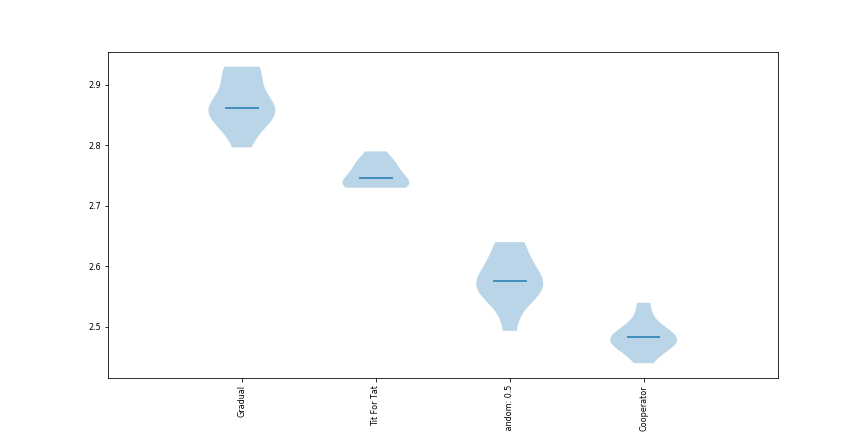
\includegraphics[width=0.5\textwidth]{../img/examples/small_violin.png}
    \caption{Ranked violin plot of the mean payoff for each player}
    \label{fig:violinplot}
\end{figure}

\begin{figure}
    \centering
    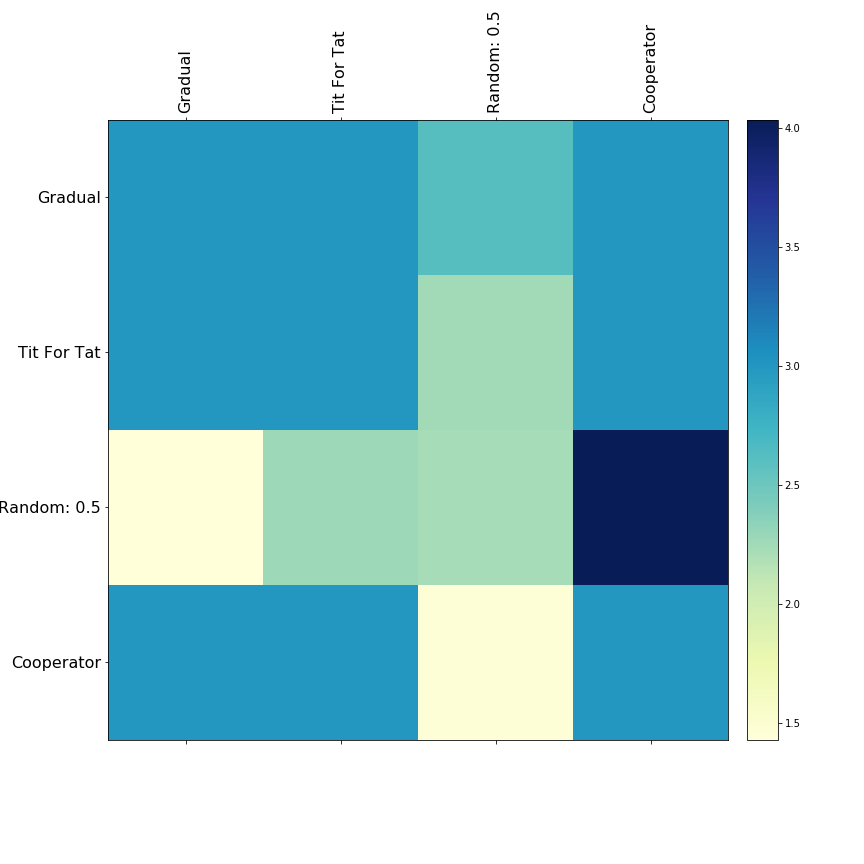
\includegraphics[width=0.5\textwidth]{../img/examples/small_payoff.png}
    \caption{Matrix plot of pair wise payoffs for each player}
    \label{fig:matrixplot}
\end{figure}

The difference in scores in Figure \ref{fig:violinplot} imply that the strategies included are all different from each other.
However, as more strategies are included it becomes harder to establish when they might be equivalent.

\section{Fingerprinting}\label{sec:fingerprinting}

The method of Fingerprinting is a technique for generating a functional signature for a strategy \cite{Ashlock2008}.
Fingerprint functions can then be compared to allow for easier identification of similar strategies.
It was first given in \cite{Ashlock2004} and has been extended in \cite{Ashlock2008, Ashlock2010,  Ashlock2005, Ashlock2009, Ashlock2006}.

In \cite{Ashlock2004} Ashlock outlines several definitions, theorems and proofs concerning the construction of a Fingerprint.
These are then followed by some examples, however they are of low quality and the only probe (see definition \ref{def:fingerprint}) used is TitForTat.

A large extension to the work is made in \cite{Ashlock2008}.
More examples are presented using 4 different probes instead of solely TitForTat, and a catalogue of several Fingerprint functions is given.
Fingerprinting is then used to to assess how three evolutionary algorithms produce different populations.
The evolutionary methods are used to train finite-state machines, lookup tables and feed forward neural nets.
Fingerprinting demonstrates that all three representations sample the strategy space in a radically different manner.

A recount of Ashlock's work in \cite{Ashlock2008, Ashlock2010, Ashlock2004,  Ashlock2005, Ashlock2009, Ashlock2006} will now be given in Chapter \ref{cha:theory}.
This culminates in an \textbf{original} result allowing his work to be broadened and applied to strategies without an FSM representation.
